结合深度信息\cite{9191119, 9429889, 9933183, 9206072, 2024hipose},仅使用RGB的方法\cite{8765585, billings2019silhonet, hybridpose}提供了更广泛的应用范围和更低的成本。

目前,高性能框架\cite{wang2021gdr, su2022zebrapose}在2D图像像素和3D物体表面顶点之间建立对应关系。然后使用一种Perspective-n-Point (PnP)算法变体\cite{EPnP}来估计姿态。对应关系通常以两种方式使用:(1) 作为辅助目标\cite{su2022zebrapose},随后应用PnP算法来估计姿态,或(2) 作为中间变量,通过网络输出姿态\cite{wang2021gdr}。然而,PnP算法需要2D和3D点之间的一对一映射,这对对称物体来说是一个挑战。例如,在一个无纹理的球体的情况下,图像中的任何像素都可以与物体表面上的任何顶点相关联。当目标对应关系由单一的真实姿态指定时,问题变得更加突出。

先前的工作\cite{pvnet, park2019pix2pose, su2022zebrapose}表明,通过使用强大但计算密集的方法,如RANSAC-PnP变体来处理高外点对应率,可以缓解对称性模糊问题。其他工作\cite{wang2021gdr, di2021so}训练端到端网络直接回归姿态参数,绕过PnP问题。然而,在严重遮挡的情况下,会出现模糊问题,导致姿态估计精度显著下降,因为对应关系预测的准确性显著下降。

\begin{figure}[t]
        \centerline{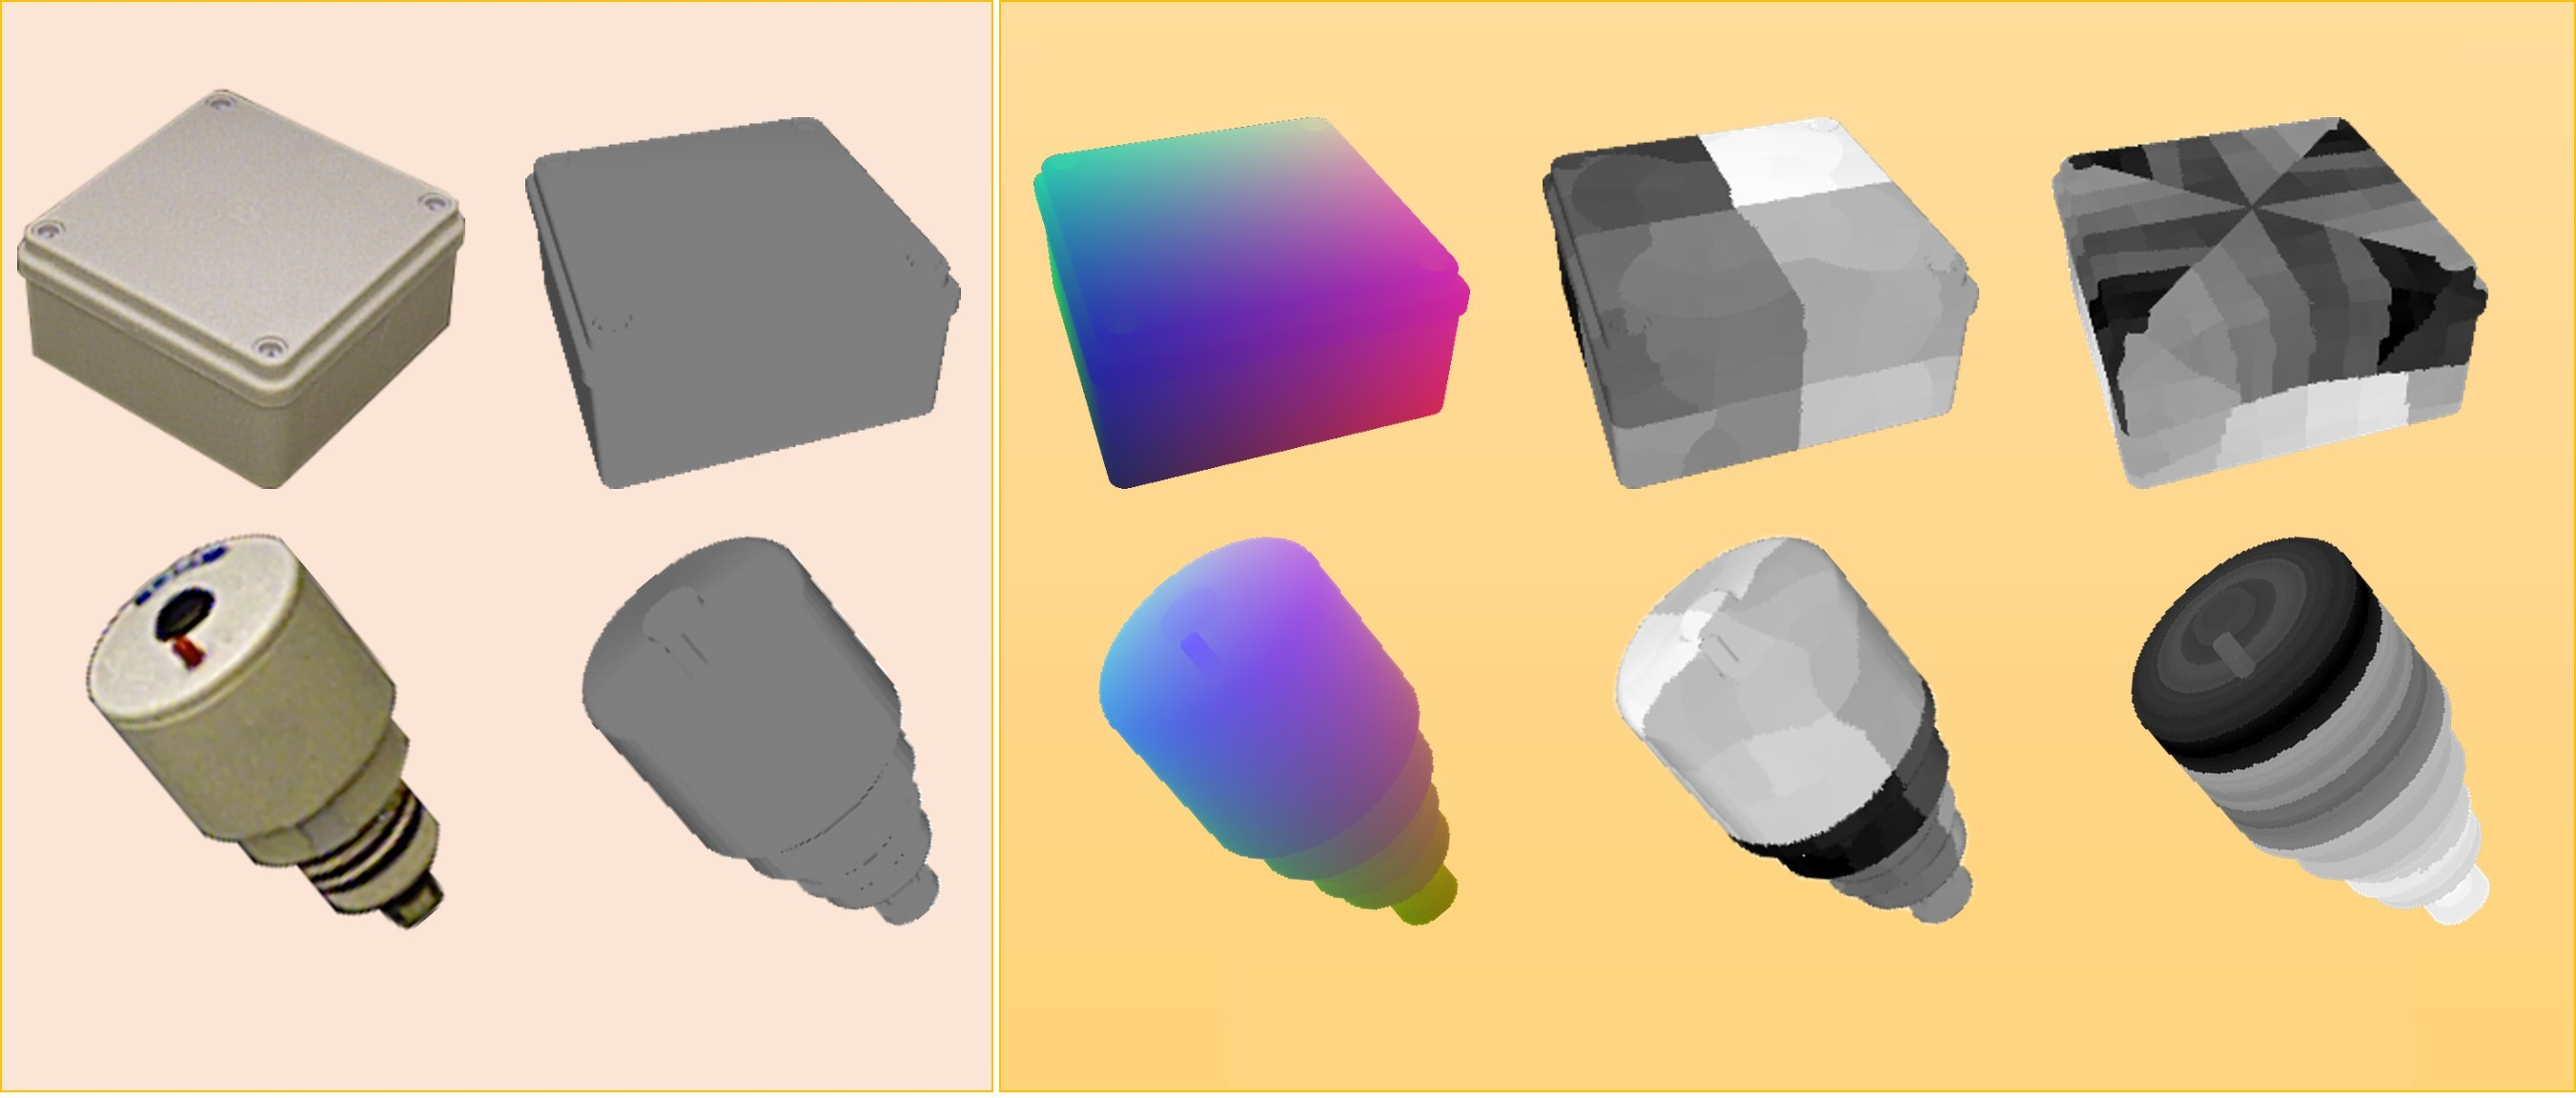
\includegraphics[width=0.90\textwidth]{figure/symnet/compare_encoder.jpg}}
        \caption{\textbf{表面编码比较。} (a) 物体图像。 (b) 无纹理模型。 (c) 3D坐标编码。 (d) ZebraPose编码\cite{su2022zebrapose}。 (e) 我们提出的SymCode。基于一对一对应关系的3D坐标编码和ZebraPose编码没有考虑对称性。相比之下,基于一对多对应关系的SymCode明确保留了对称性信息。}
        \label{compare_encoder}
\end{figure}